\section{一维数组}
在前面的章节中,我们用各种数据类型、运算符和选择结构,可以处理一些小规模的问题。循环结构允许我们用少量的代码处理一些规模较大的问题,但是我们所掌握的数据方面的知识太少,还没有跟得上这样突飞猛进的处理能力。试想,如果我们需要100个变量来存储不同信息,并在我们需要时对它进行处理,那么``如果把这100个变量存下来''就成了我们的难题。我们要定义100个变量吗?这样写起来好像也很麻烦吧。而且更可怕的是,如果我们也不能确定需要多少个数据(可能100个,或者100000个),那怎么办?我们要怎么搞到这么多变量名啊?\par
且慢。我在本章中一再提醒读者,变量名并不是变量的本质。如果要读取或者存储某个变量的信息,我们是可以不需要变量名的。假如说现在有三个 \lstinline@float@ 型的变量(每个变量占4字节内存),我暂且用 \lstinline@a@, \lstinline@b@, \lstinline@c@ 来称呼它们,如果它们在内存中的地址是挨着的,比如图5.10中的这种情况,我们可以定义一个 \lstinline@float*@ 类型的指针 \lstinline@pf=&a@,让它指向 \lstinline@a@。\par
\begin{figure}[htbp]
    \centering
    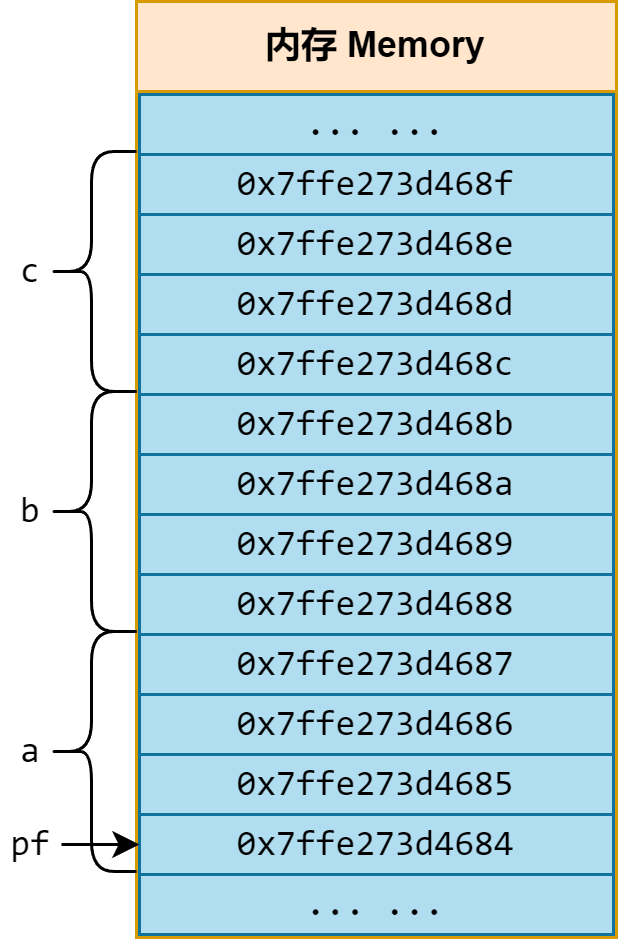
\includegraphics[width=0.4\textwidth]{../images/generalized_parts/05_variables_one_by_one_in_memory.png}
    \caption{如果三个变量在内存中的地址是挨着的,我们可以用一个指针来访问这三个数据}
\end{figure}
接下来我们就可以用这一个指针访问这三个数据。还记得我们讲过指针的运算吧,\lstinline@pf+1@ 相对于 \lstinline@pf@ 偏移了一个数据(而非一个字节)。既然 \lstinline@pf@ 是 \lstinline@a@ 的地址,那么 \lstinline@pf+1@ 就是 \lstinline@b@ 的地址,\lstinline@pf+2@ 就是 \lstinline@c@ 的地址。\par
试想一下,如果有100个同类型数据,它们都是紧挨着的,那么我们用一个指针 \lstinline@p@ 指向第一个元素,那接下来不就可以用 \lstinline@p+index@ 表示第 \lstinline@index+1@ 个数据的地址了吗?\footnote{注意,\lstinline@p+0@ 是第一个数据的地址,所以以此类推,\lstinline@p+index@ 是第 \lstinline@index+1@ 个数据的地址。}\par
不过C/C++标准从来就没有保证过``连续定义的若干变量在内存中必须是紧挨着的''。所以我们需要一点点手段来确保这个前提——这就是\textbf{数组(Array)}。\par
本节我们先来介绍一维数组,高维数组留待后面再讲。\par
\subsection*{一维数组的定义和使用}
数组是一大类复合类型,它可以用于批量定义数据。定义一个数组的基本的语法是
\begin{lstlisting}
    <类型> <数组名>[<数组长度>] = {<初始化列表>};
\end{lstlisting}
其中的长度是一个 \lstinline@size_t@ 类型的常量表达式\footnote{现代编译器大都支持数组定义时使用非常量的长度,此时编译器会用一套比较复杂的机制来创建这个数组。但是我仍建议读者在需要使用动态大小的数组时选择动态内存分配语法。}。话虽这么说,但因为整型数据都可以隐式类型转换成 \lstinline@size_t@ 类型,所以我们直接用整型的常量表达式来定义就可以。\par
以下是一些正确的定义方式:
\begin{lstlisting}
    double array1[3] = {1e5, .3, -1}; //正常格式,可省略=号
    int array2[4] {1}; //省略部分或全部内容,省略的部分使用默认值(0)
    float array3[] {0.1f, 0.2, 0.3d}; //省略长度,数组长度会被定为{}内的数据个数
\end{lstlisting}
而以下的定义方式是错误的:
\begin{lstlisting}
    int array4[3] {1, 2, 3, 4, 5}; //初始化列表中的数据个数超过长度限制
    int array5[5] {1, , , ,1}; //不能略过中间的数据,定义后面的数据
    int array6[] {}; //C++标准禁止使用长度为0的数组
\end{lstlisting}
数组是什么类型呢?看上去好像很神秘,但如果我们试着输出这个数组的名字,就会发现,它输出的东西很像是一个地址值\footnote{字符型的数组依然是一个例外,我们会在后面讲到它。}。
\begin{lstlisting}
    cout << array1; //输出0x7fff32b2044c或者别的,总之很像一个地址
\end{lstlisting}\par
事实上,在我们日常使用数组的过程中,大部分情况下数组类型都会隐式类型转换成对应类型指针。刚才的输出语句就是一例,在输出之前,\lstinline@double[3]@ 类型的 \lstinline@array@ 会被隐式类型转换为 \lstinline@double*@ 类型,然后作为一个地址值输出。\par
在涉及加减法时亦如此。\lstinline@array2@ 原本是 \lstinline@int[4]@ 类型的,而在与整型数据进行加减时,就会先隐式转换成 \lstinline@int*@ 类型,然后作为一个指针来进行加减。\par
不难发现,数组正好有我们在本节开头中所希望的那种性质:其一,一个数组包含了若干连续数据,它们紧挨着排布;其二,数组名可以视作一个指针,我们可以用 \lstinline@p+index@ 的形式来读取或修改它的值。\par
那么如果我要定义一个大小为100的 \lstinline@int@ 数组,并把每个值都变成 \lstinline@0@,我可以如何做呢?
\begin{lstlisting}
    int array[100] {}; //{}的中省略了全部的初始化,这样每个数据都会初始化为0
\end{lstlisting}\par
如果我要定义一个大小为10000的 \lstinline@int@ 数组,并把每个值都变成 \lstinline@1@,我又该如何做呢?这里不太一样,我们无法用简洁的语法直接把所有数据都初始化为1,所以需要另想方法。这里我们可以用 \lstinline@for@ 循环来批量处理这些数据,这时就能体现出循环语句的强大了。
\begin{lstlisting}
    int array[10000]; //无需初始化,反正待会就要赋值
    for (int i = 0; i < 10000; i++) //注意循环的起止条件
        *(array + i) = 0; //array+i即是第i+1个数据的地址,再取内容,就可以修改了
\end{lstlisting}
注意,\lstinline@array@ 是第一个数据的地址,所以 \lstinline@array+1@ 是第二个数据的地址,……,以此类推,第10000个数据的地址应该是 \lstinline@array+9999@。因此在这里我们需要控制循环的起始和终止条件,让 \lstinline@i@ 从 \lstinline@0@ 开始,到 \lstinline@9999@ 终止\footnote{虽然我们可以访问 \lstinline@array+10000@,但我们无法保证这个空间是安全的。换言之,使用\lstinline@array+10000@ 会带来类似于野指针的问题。}。\par
用 \lstinline@*(array+i)@ 这样的方式来访问显得有点麻烦了。在C/C++中,我们还有一种方式可以访问数组的数据,那就是用下标运算符 \lstinline@[]@ 来实现这个功能。在C/C++中,如果 \lstinline@arr@ 是一个数组类型,那么我们可以用 \lstinline@arr[i]@ 的方式来替代 \lstinline@*(arr+i)@,效果相同。这个语法还可以扩展到指针层面,如果 \lstinline@p@ 是一个指针,我们也可以用 \lstinline@p[0]@ 的方式来替代 \lstinline@*p@。\footnote{实际上,对于数组名或指针来说,\lstinline@p[i]@ 形式的表达式都会被编译器当作\lstinline@*(p+i)@ 来处理,所以这么写只是会让我们自己方便一点而已,对于编译器来说没会么区别。}\par
\begin{figure}[htbp]
    \centering
    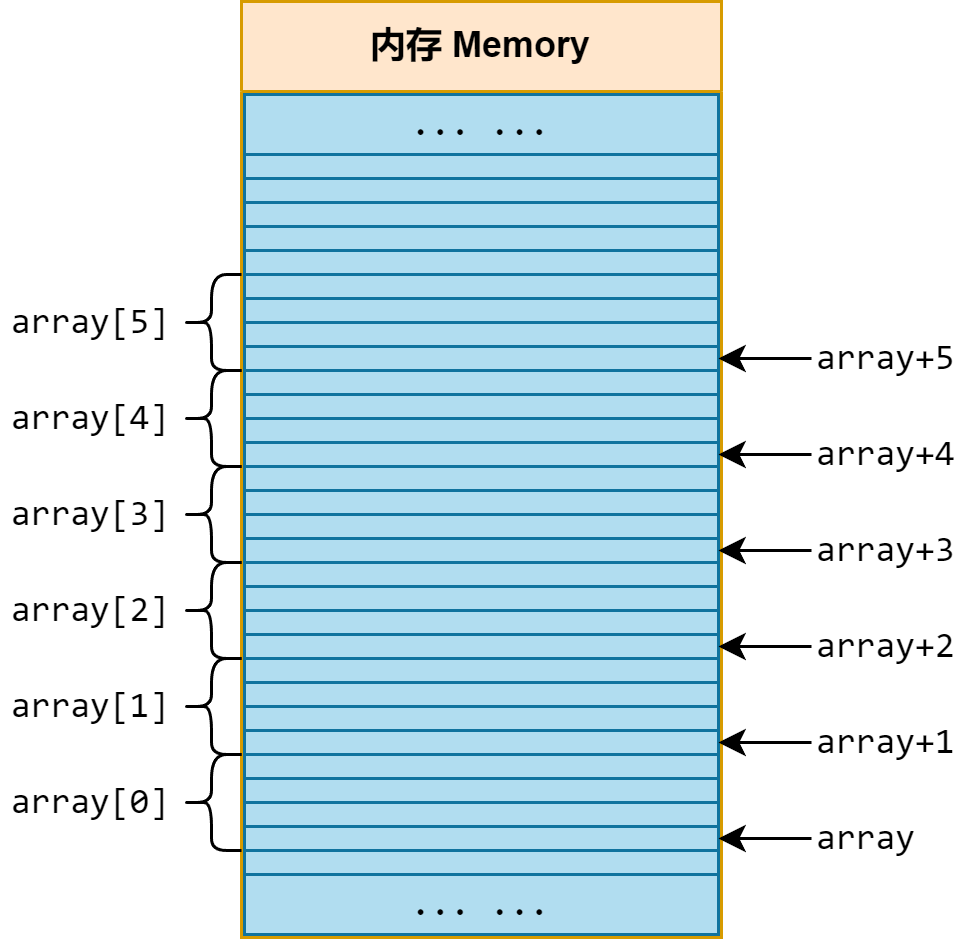
\includegraphics[width=0.6\textwidth]{../images/generalized_parts/05_variables_one_by_one_in_array.png}
    \caption{用 \lstinline@array[i]@ 效果等同于 \lstinline@*(array+i)@}
\end{figure}
有了数组之后我们就可以只需要一个名字 \lstinline@array@,然后通过下标来读取或修改大量数据了。当然,不要忘记数组下标是从 \lstinline@0@ 开始的,所以 \lstinline@array@ 数组的第一个数是 \lstinline@array[0]@ 而不是 \lstinline@array[1]@。下面是一个对数组中各数字进行求和的例子,我们需要用户先输入 \lstinline@10@ 个数,然后求出它们的和。
\begin{lstlisting}
    int arr[10], sum {0}; //定义一个数组arr和int数据sum,sum初始化为0
    for (int i = 0; i < 10; i++) //注意条件
        cin >> arr[i]; //输入arr[i]的值,arr[i]是arr数组第i+1个数
    for (int i = 0; i < 10; i++)
        sum += arr[i]; //用加赋值运算符,把arr[i]的值加到sum中
    cout << "总计:" << sum;
\end{lstlisting}
我们可以试一下这段代码的运行效果:\\\noindent\rule{\linewidth}{0.2pt}\texttt{
\textbf{1 2 3 4 5 6 7 8 9 10}\\
总计:55
}\\\noindent\rule{\linewidth}{0.2pt}
它的运行结果也很符合我们的预期。\par
\subsection*{数组参数传递}
我们在前面写了一个 \lstinline@maximum@ 函数模板,它可以求两个数的最大值。现在我们想要求大量数据的最大值,再用 \lstinline@maximum@ 重载的方法就显得太不合适了(即便我们有一个能传递任意数量参数的函数,我们也要衡量一下调用的时候是不是要把一个个参数全都写进去)。为了解决这个问题,我们需要考虑能否用数组来实现这个功能。\par
在C++中,我们可以传递一个数组的首地址,作为函数的参数。这里``数组的首地址'',指的就是数组在内存空间中的第一个字节对应的地址。从地址值上讲,它就等于 \lstinline@&array[0]@——我们之后再来谈它们在类型上的区别,目前读者这样理解就足够了。\par
以下是一个实现此功能的代码,可以接收5个浮点数输入,然后给出其中最大的数。读者可以先试着运行它,然后我将分别对语法和语义进行讲解。
\begin{lstlisting}
template<typename T>
T maximum(T arr[], unsigned n) {
    T res {arr[0]}; //先假设最大值为arr[0]
    for (int i = 1; i < n; i++)
        if (arr[i] > res) //如果arr[i]>res,说明有更大的数
            res = arr[i]; //那么目前能找到的最大值就是arr[i]
    return res; //res就是返回值
}
int main() {
    double arr[5]; //定义一个数组arr和int数据sum,sum初始化为0
    for (int i = 0; i < 5; i++)
        cin >> arr[i];
    cout << maximum(arr, 5); //传入arr数组,并告诉这个函数arr有多大
    return 0;
}
\end{lstlisting}\par
从语法上,我们可以看到,\lstinline@maximum@ 是一个函数模板,它可以接收一个 \lstinline@arr@ 数组和一个 \lstinline@n@ 无符号整数作为参数。你可能会好奇,为什么我们要把形参写成 \lstinline@arr[]@ 的形状呢?写成 \lstinline@arr[5]@ 不行吗?\par
可以,但没有意义。在数组参数传递的过程中,我们传递的不是数组本身,而是它的首地址——换句话说,传递的是一个指针。在编译器进行编译的时候,它会把 \lstinline@T arr[]@ 参数视同 \lstinline@T *arr@,所以即便我们在 \lstinline@arr[]@ 中写了 \lstinline@5@,也会被忽略,没有意义。\par
也正因为数组参数传递过程中只传递了指针,所以函数不能判断这个数组的大小,因此我们必须再加一个参数,来描述这个数组的大小。这就是 \lstinline@n@ 存在的意义。\par
再来看语义,\lstinline@maximum@ 函数中的这段代码是如何做到我们希望的功能的呢?其实就是用 \lstinline@for@ 循环读取 \lstinline@arr@ 中的每个数,然后逐一比较。如果发现了一个更大的数,那就说明最大值至少应该是这个数,所以 \lstinline@ref=arr[i]@ 赋值一下。如果之后又发现了一个更大的数,那就说明最大值至少应该是这个数,所以 \lstinline@ref=arr[i]@ 再赋值。这样一直找到最后,\lstinline@res@ 就是所有数的最大值了。读者若是还未明白,可以把自己想像成程序,以输入 \lstinline@2,1,4,5,3@ 为例,模拟一下这个过程。\par
有些时候,我们也不知道输入数据有多少个\footnote{这种情况最常见于字符串的输入。},那么怎么办呢?为了不出问题,我们可以设计一个尽可能大的数组(比如,大小为1000的数组 \lstinline@arr@) ,然后让用户输入尽可能多的数据。如果用户输入了字母 \lstinline@q@ 或者类似的不合理内容,就结束输入循环。这个思路与\hyperref[lst:OddOrEvenWithWhileLoop]{代码3.3}的判断方式很相似。\par
我们还需要考虑一种情况,用户的输入可能超过1000个,这时如果不加防范,程序会继续将输入存到 \lstinline@arr[1000]@, \lstinline@arr[1001]@ 这些地方。这会造成野指针问题,不得不防范!所以我们还需要在循环时判断一下,数组下标是否越过了边界。\par
鉴于此,我们可以写一个输入函数。我们可以用 \lstinline@for@ 循环或者 \lstinline@while@ 循环,实现的方式也可以有细微不同,只要能以简单高效的方式达到我们的目的就好。
以下是第一种写法:
\begin{lstlisting}
    double arr[1000]; //为了能接收任意数量的输入,预先设置一个比较大的数组
    unsigned size = 0; //定义一个size变量,用来表示数组中目前的数据量
    for (; size < 1000 && cin; size++) { //注意判断条件
        cin >> arr[size]; //输入到arr[size]中,然后size会自增
    }
    cout << maximum(arr, size); //现在是长度为size的arr数组,传入函数中
\end{lstlisting}
这里使用 \lstinline@for@ 循环,其中的判断条件是个逻辑与表达式。之所以用 \lstinline@size<1000@ 而不是 \lstinline@size<=1000@ 是因为,条件判断是在输入 \lstinline@arr[size]@ 之前进行的,而迭代是在输入之后进行的。如果某次 \lstinline@size@ 的值为 \lstinline@999@,那么本次判断可能为 \lstinline@true@,输入正常进行,输入了 \lstinline@arr[999]@ 之后,\lstinline@size@ 才迭代为 \lstinline@1000@。而如果某次 \lstinline@size@ 的值为 \lstinline@1000@ 了,这时倘若用 \lstinline@size<=1000@ 来判断,那就会出现 \lstinline@arr[1000]@,这就越界了!\par
我们还可以使用 \lstinline@while@ 语句来实现,思路大同小异。\par
我们也可以把这个输入功能做成函数,就叫 \lstinline@input_arr@,它接收一个数组参数(其实是指针参数),再接收一个数组容量参数(这个数组最大的容量是多少)。考虑到用户的输入未必能达到最大值(``容量''与``实际储量''当然不一定相同),我们还需要知道这个数组实际装了多少数据。我们可以把这个数据作为 \lstinline@input_arr@ 的返回值。\par
这个思路比较清晰,我们可以直接写一个这样的函数出来:
\begin{lstlisting}
template<typename T>
unsigned input_arr(T arr[], const unsigned max_size) {
    unsigned real_size {0}; //记录数组中数据的实际个数
    while (real_size < 1000) { //防止数组下标越界
        cin >> arr[real_size]; //输入arr[real_size]
        if (!cin) { //如果输入状态错误
            input_clear(); //先清理输入
            break; //再退出while循环
        }
        ++real_size; //然后real_size自增
    }
    return real_size;
}
\end{lstlisting}
这个函数略显复杂,注意事项也比较多,我们慢慢道来。\par
首先,它是一个函数模板,会根据我们的需要生成对应类型的函数实例。这里没什么可说的。\par
\lstinline@max_size@ 是数组最大容量。它只是一个副本,我们改动它也不会影响原变量,但是我依然建议使用 \lstinline@const@,以避免在函数中误修改它的值。至于数组传递,它本身就是一种指针传递,所以我们直接在 \lstinline@input_arr@ 函数中修改 \lstinline@arr@ 数组的数据就行了,而不需要什么所谓``对数组的引用''。\par
在 \lstinline@while@ 语句中我们只判断 \lstinline@real_size@ 是否越界。而对于异常输入的情况,我们选择使用 \lstinline@if(!cin)@ 判断加 \lstinline@break@ 语句来退出循环。\par
语法正确还不够。你还需要考虑清楚 \lstinline@while@ 循环中各语句的执行顺序,以免出现语义错误。例如 \lstinline@++real_size@ 这一句,必须要在 \lstinline@if(!cin)@ 之后,这两句的顺序是不能调换的。这是因为,只有当 \lstinline@cin@ 正常的时候,\lstinline@arr[real_size]@ 才能得到有效输入,这时 \lstinline@real_size@ 才应该自增;否则,\lstinline@arr[real_size]@ 得不到有效输入,\lstinline@real_size@ 也不该自增,所以应当直接用 \lstinline@if(!cin)@ 中的 \lstinline@break@ 语句退出这个循环,避免执行 \lstinline@++real_size@。\par
接下来我们可以使用这个函数,配合 \lstinline@maximum@ 来实现先输入,后求最大值的功能了。\par
\begin{lstlisting}
int main() {
    int arr[1000];
    unsigned arr_size {input_arr(arr, 1000)};
    //向arr提供输入,并由arr_size接收返回值,记录当前arr数组中的有效数据个数
    cout << maximum(arr, arr_size);
}
\end{lstlisting}\par
如果我们发现用户实际输入的需求可能是几万个,而非几个到几百个,那我们就要考虑增加 \lstinline@arr@ 的容量。我们可以把定义句改为 \lstinline@int arr[100000]@。\par
这就完了吗?不,还没有,我们还需要改 \lstinline@input_arr(arr,1000)@ 这里的参数呐!把它也改成 \lstinline@100000@ 才行。\par
这就体现出单纯用字面量的缺点了,我们没法保证一次修改之后所有相关数据都改变,而人为操作的话,出现遗漏和失误的可能性又太大了。为了保持统一性,我们可以用常量或常量表达式,通过具名的方式把数组的容量描述出来。
\begin{lstlisting}
    constexpr int Maxsize {100000}; //用const也可
    int arr[Maxsize];
    unsigned arr_size {input_arr(arr, Maxsize)}; //这样就好了
\end{lstlisting}
这样,如果我们需要改 \lstinline@Maxsize@ 的值,只要修改一次,就可以把所有需要改的数据一并改完了,犯错的可能性大大降低。\par
关于输入和求最大值,我们还可以有一些更有技巧性的写法:
\begin{lstlisting}
    const int Maxsize {100000}; //用constexpr也可
    int arr[Maxsize];
    cout << maximum(arr, input_arr(arr, Maxsize)); //?
\end{lstlisting}
在这里,我们是把输入和求最大值并到同一步来写了。这句可能有点乱,但我们分析一下就会发现它很好懂。\par
首先,\lstinline@maximum@ 接收两个参数,一个是 \lstinline@arr@,而另一个是 \lstinline@input_arr(arr,Maxsize)@。这也就是说,我们需要把 \lstinline@input_arr@ 的返回值求出来,然后才能执行 \lstinline@maximum@ 函数。而在 \lstinline@input_arr@ 执行过程中,程序会先进行输入(这是 \lstinline@input_arr@ 函数的副作用),然后返回实际存储数据的个数。这个个数将作为参数被 \lstinline@maximum@ 函数使用。\par
下一步,\lstinline@maximum@ 知道了 \lstinline@arr@ 数组的位置和实际数据的个数,然后就会在对应的范围中求出最大的数。这时的 \lstinline@arr@ 也已经保存了用户输入的值(这是 \lstinline@input_arr@ 的副作用),所以整个程序就这样顺理成章地运行下去了。\par
\lstinputlisting[caption=\texttt{输入数据求最大值.cpp},label=lst:GetMaximumFromInput]{../code_in_book/5.1/输入数据求最大值.cpp}\par
这应该是本书迄今为止展示的最长代码了,但是关于它的每个部分,我都已经拆解过(除了 \lstinline@input_clear@,这部分我们暂且不讲,读者知道怎么用即可)。当我们想要实现较复杂的功能时,长代码总是难以避免的。这也正是我们需要用函数来进行``模块化''的一个重要原因。\par
\subsection*{范围 \lstinline@for@ 循环}
有的时候我们可能需要对一个数据的数据进行批量处理,这时我们一般用 \lstinline@for@ 循环来实现。好处也很明显,\lstinline@for@ 循环内部可以定义一个下标变量 \lstinline@i@(或者用别的名字),终止条件可以通过比较运算来实现,而迭代操作刚好可以处理下标的变化。这样看来,\lstinline@for@ 循环仿佛是为数组处理量身打造的。\par
从C++11标准起,范围 \lstinline@for@ 循环(Range-based for loop)能让我们一次性读取(或修改)数组中所有数据的操作变得更简单。比如说,我们定义一个数组,然后输出它的所有数据,可以这样写:
\begin{lstlisting}
    int arr[] {1,2,3}; //定义一个长度为3的数组
    for (int x : arr) //用范围for循环,变量x接收arr中的数据
        cout << x << ' '; //输出x的值
\end{lstlisting}
这样一来,范围 \lstinline@x@ 就会循环接收 \lstinline@arr@ 中的每个数字,然后在循环体内进行操作。\par
如果我们要修改它的值呢?把 \lstinline@x@ 定义成 \lstinline@int@ 类型的变量是不行的,因为它相当于一个临时变量。因此我们需要使用引用来实现修改的功能。
\begin{lstlisting}
    int arr[] {1,2,3,4}; //定义一个长度为4的数组
    for (int &x : arr)
        x *= x; //将x的值变为原数的平方
\end{lstlisting}
这个范围 \lstinline@for@ 循环看上去很好用,不过它也存在较多的限制:
\begin{itemize}
    \item 范围 \lstinline@for@ 循环会对数组中的所有数据进行处理,我们无法人为改变它的处理范围。这也就意味着,如果某个数组中的数据不都是有效数据,那么这种方法可能会把无效数据一并处理。比如说,输出了不该输出的部分,或者是把不该平方的数据也给平方了。即便这样做不会带来任何危险,它也会在实际运行的过程中带来效率问题(因为我们把一些时间浪费在了不该处理的数据上)。
    \item 范围 \lstinline@for@ 循环不能处理那些``看上去是数组,但实际是指针''的东西。\footnote{这是因为,指针相比于数组,缺少了``数组长度''这条信息,所以范围 \lstinline@for@ 循环根本不能确定数组的实际大小。详见后文。}比如说,函数中接收的``数组参数'',其实它们全都是指针。那也就意味着,代码5.1中的 \lstinline@maximum@ 和 \lstinline@input_arr@ 都是无法使用范围 \lstinline@for@ 循环的。我们在后面接触动态内存分配时也会发现这个问题,动态数组不能使用范围 \lstinline@for@ 循环来处理数据。
\end{itemize}
\subsection*{数组的类型}
那么数组和指针之间到底是什么关系呢?为什么数组就可以用范围 \lstinline@for@,指针就不能?为什么数组名可以隐式类型转换成指针?\par
如果我们用 \lstinline@is_same@ 来比较一个数组类型和一个指针类型,就会发现它们确实是不相同的。
\begin{lstlisting}
    int arr3[3], int *p;
    cout << is_same<decltype(arr3), decltype(p)>::value; //输出为0
\end{lstlisting}\par
那么我们试试比较一下两个长度不同的数组类型呢?
\begin{lstlisting}
    int arr3[3], arr5[5];
    cout << is_same<decltype(arr3), decltype(arr5)>::value; //输出也为0
\end{lstlisting}
哎,看起来这两个类型也不相同。\par
没错,数组类型的区分比指针更细。对于指针来说,指向\lstinline@int@ 的指针当然和指向 \lstinline@long long@ 的指针是不同类型,但是任何两个指向 \lstinline@int@ 的指针都是同类型的。\par
数组不然,不光数据类型不同的数组不是同类型,连长度不同的数组也不是同类型了。这里的 \lstinline@arr3@ 的真实类型应该是 \lstinline@int[3]@ 型,而 \lstinline@arr5@ 的真实类型应该是 \lstinline@int[5]@ 型。\par
可惜 \lstinline@is_same@ 在这里能告诉我们的信息还是太少了,我们只能知道``某两个类型具体是什么'',但还不情楚``某个类型意味着什么''。所以我们还有另一个工具,那就是 \lstinline@typeid@ 运算符。\par
\lstinline@typeid@ 有点像 \lstinline@sizeof@,它既可以作用于类型,又可以作用于对象(变量)。\lstinline@typeid@ 的成员函数 \lstinline@name()@ 可以返回一个 \lstinline@const char*@ 对象(这是一个字符串,详见下一节)。我们输出它,就可以看到相关的类型信息了。以下是一个示例:
\begin{lstlisting}
    int arr3[3], arr5[5];
    cout << typeid(arr3).name() << endl;
    cout << typeid(arr5).name() << endl;
    cout << typeid(int).name() << ' ' << typeid(double).name() << ' '
        << typeid(unsigned).name() << ' ' << typeid(float).name() << endl
        << typeid(int*).name() << ' ' << typeid(char*).name();
\end{lstlisting}
需要提醒读者,\lstinline@typeid(...).name()@ 在不同编译环境下的结果可能不同\footnote{实际体验是,在MSVC开发环境中给出的结果最为清晰。},因此本例中的结果取Coliru上运行的结果。读者也可以在Coliru上自行运行这段代码试试效果。它的输出是\\\noindent\rule{\linewidth}{.2pt}\texttt{
A3\_i\\
A5\_i\\
i d j f\\
Pi Pc
}\\\noindent\rule{\linewidth}{.2pt}\par
其中 \lstinline@A3_i@ 格式的内容表示一个长度为3的 \lstinline@int@ 型数组(Array),\lstinline@A5_i@ 表未一个长度为5的 \lstinline@int@ 型数组。\par
而接下来的 \lstinline@i@, \lstinline@d@ 等分别是 \lstinline@int@, \lstinline@double@ 等类型的名字。\par
最后输出的 \lstinline@Pi@ 和 \lstinline@Pc@ 分别是两个指针类型的名字,其实就是在原类型名字前面加上了 \lstinline@P@ ,代表指针(Pointer)。\par
\begin{figure}[htbp]
    \centering
    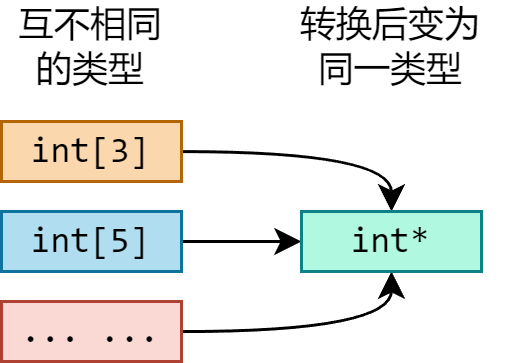
\includegraphics[width=0.3\textwidth]{../images/generalized_parts/05_array_to_pointer_conversion.png}
    \caption{数组到指针的类型转换}    
\end{figure}
也就是说,数组比指针多出了一个``长度''信息。虽然我们一般看不出这个信息来,但是它确实存在。不信的话,你还可以用 \lstinline@sizeof@ 取数组的内存空间大小看一下,它是不是与数组长度挂钩。
\begin{lstlisting}
    int arr3[3], arr5[5];
    cout << sizeof arr3 << endl << sizeof arr5;
\end{lstlisting}
而指针不是这样的。指针也是变量,它在内存空间中也有对应的存储位置\footnote{因此我们还可以取一个指针的地址,这是后话。}。我们可以用 \lstinline@sizeof@ 计算一下。\par
那么来到数组参数传递这里——我们也可以用 \lstinline@typeid@ 取``数组形参''的类型,或者用 \lstinline@sizeof@ 来取它的内存空间大小,就会发现它的表征和指针是一样的:
\begin{lstlisting}
void fun(int arr[]) {
    cout << typeid(arr).name() << ' ' << sizeof arr;
    //输出Pi 8,说明arr是一个指针!
}
int main() {
    int arr[1000];
    fun(arr);
}
\end{lstlisting}\par
所以说数组参数传递看似是在传递数组,其实是在传递指针。而在传递的过程中,数组原本所含有的``长度''信息就丧失了,因此我们在传递数组的过程中,最好要另外加上一个参数,说明一下数组的长度,否则函数也不能确定数组的长度,就难免会发生下标越界问题。\par
